% Section content template for individual Educative lessons
% This file contains the actual content for a specific section
% Generated from Educative API section content

% Section: SOLID: Single Responsibility Principle
% Section ID: 6062503710949376
% Section Slug: solid-single-responsibility-principle
% Generated: 2025-12-11T05:49:53.591954

\subsection{Introduction}\label{gWsMTz21fmqwN7T7VLVcC-1}
\\
The \textbf{Single Responsibility principle (SRP)} is perhaps the least understood SOLID concepts. Robert C. Martin coined the term and defines it as follows: ``\emph{A class should have only one reason to change}.'' This implies that any class or component~in our code should only have one functionality. Everything in the class should be related to just one goal.
\\
When programmers need to add features or new behavior, they frequently integrate everything within the current class. When something needs to be changed later, due to the complexity of the code, the update process becomes extremely time-consuming and tedious. The Single Responsibility Principle helps us create simple classes that perform just one task. This makes making modifications or adding extensions to the existing code much easier.

\subsection{Real-life example}\label{s-B-ioRboviaKUlpFx9pZ}
\\
The following illustration represents how SRP is applied in real life:

\begin{figure}[htbp]
 \centering
 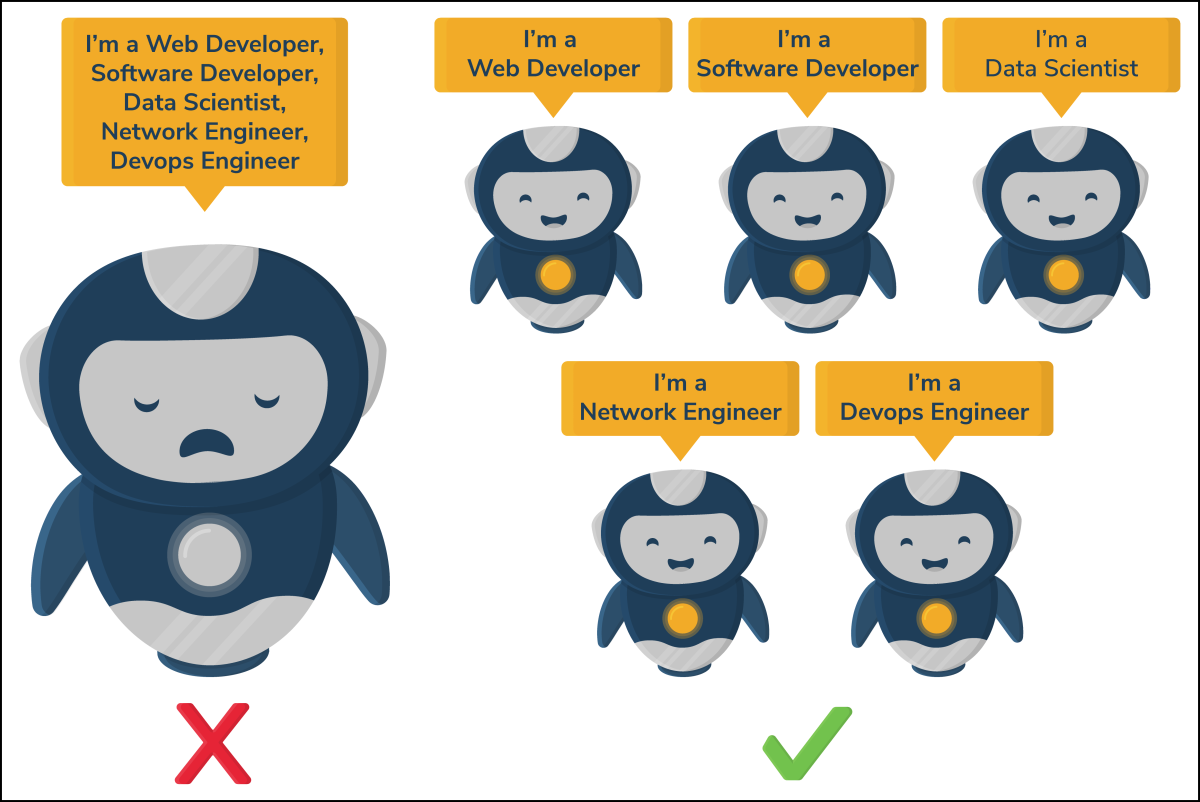
\includegraphics[width=0.5\textwidth]{Images/chapter_4/section_6062503710949376/6513474772664320.png}
 \caption{An example of SRP}
\end{figure}

\subsection{Book invoice application}\label{gWsMTz21fmqwN7T7VLVcC-2}
\\
Let's try to understand SRP with the help of an example. We have a book invoice application that has two classes: \texttt{Book} and \texttt{Invoice}. The
\texttt{Book} class contains the data members related to the book. Whereas
, the \texttt{Invoice} class contains the following three functionalities:

\begin{itemize}
\item
\protect\phantomsection\label{simSo-NwfLo15kUzeXTSt}
Calculating the price of the book.
\item
\protect\phantomsection\label{rPXDdFznXbTp6OBsvUmK0}
Printing the invoice.
\item
\protect\phantomsection\label{fxeCKVpi4bUdi3HFQurgT}
Saving the invoice into the database.
\end{itemize}
\\
The following class diagram provides a blueprint of these classes:

\begin{figure}[htbp]
 \centering
 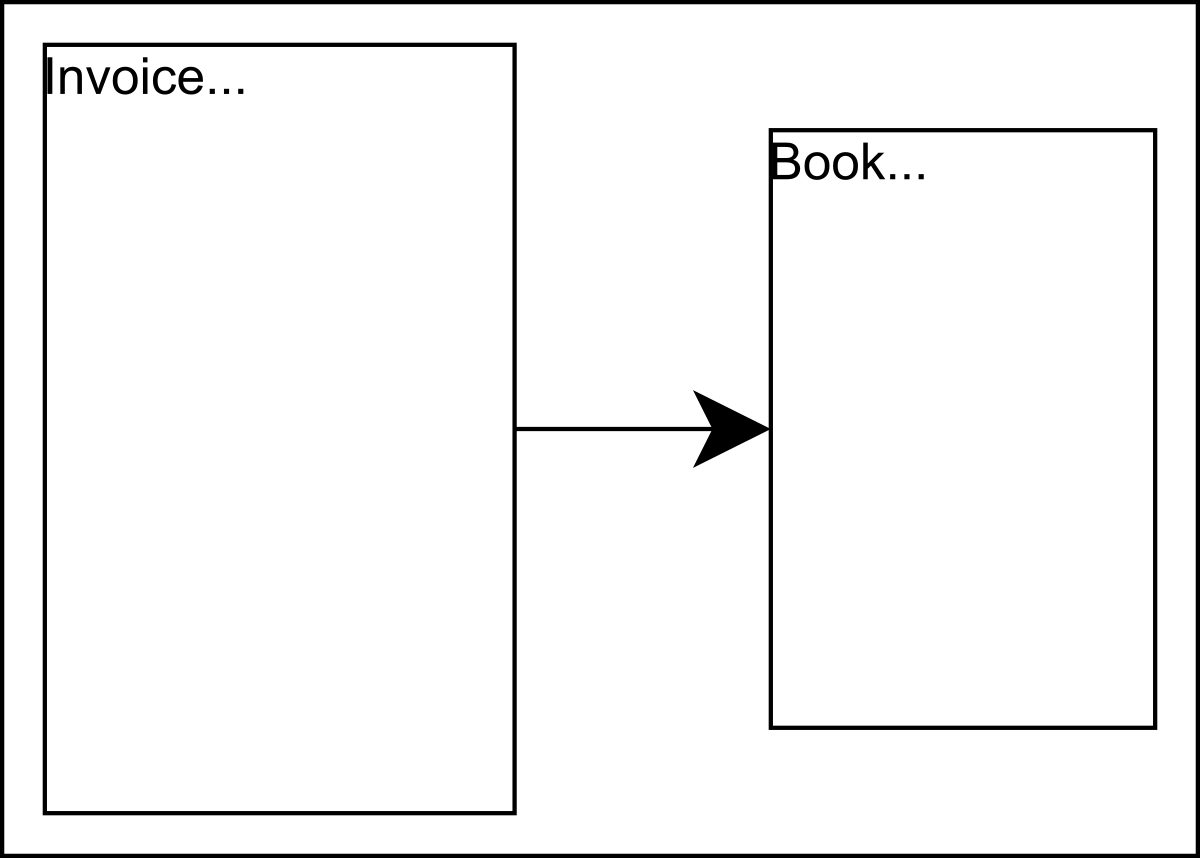
\includegraphics[width=0.5\textwidth]{Images/chapter_4/section_6062503710949376/6601944488083456.png}
 \caption{The class diagram of the book invoice application without applying the SRP rule}
\end{figure}

\subsubsection{Violations}\label{N4z6sabw6PVZHPzQaEwyG}
\\
If we notice, the\texttt{Invoice} class violates the SRP in multiple ways:

\begin{itemize}
\item
\protect\phantomsection\label{yKxsNFl73GUlXudqLgzo-}
The \texttt{Invoice} class is about invoices, but we have added print and storage functionality inside it. This breaks the SRP rule, which states, ``A class should have only one reason to change.''
\item
\protect\phantomsection\label{dKRvgWWy-zDknCH6VnIaP}
If we want to change the logic of the printing or storage functionality in the future, we would need to change the class.
\end{itemize}
\\
Instead of modifying the \texttt{Invoice} class for these uses, we can create two new classes for printing and persistence logic: \texttt{InvoicePrinter} and \texttt{InvoiceStorage}, and move the methods accordingly, as shown below.

\begin{figure}[htbp]
 \centering
 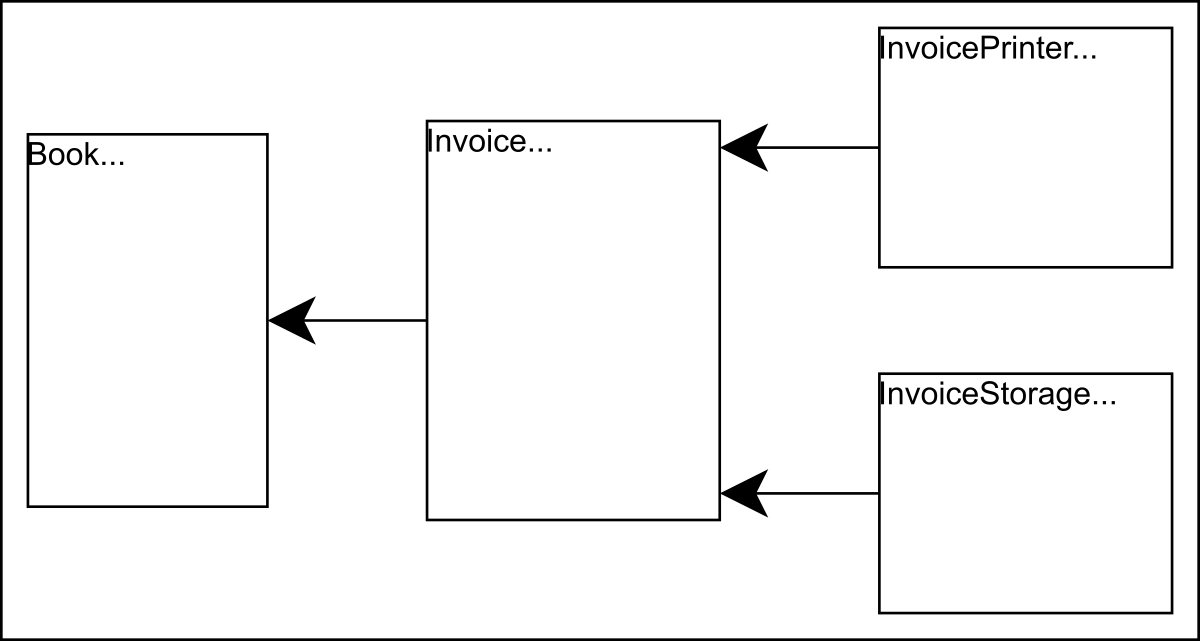
\includegraphics[width=0.5\textwidth]{Images/chapter_4/section_6062503710949376/4960364098355200.png}
 \caption{The class diagram of the book invoice application after applying the SRP rule}
\end{figure}

Now, our class structure is in line with the SRP.

\subsection{Conclusion}\label{hG2zWqLL-pb5SGdZw8IN7}
\\
When a class performs one task, it contains a small number of methods and member variables that are self-explanatory. SRP achieves this goal, and due to this, our classes are more usable, and they provide easier maintenance.
\\
In the next lesson, we will learn the Open/Closed design principle with examples.

% End of section content